\documentclass[tikz,border=10pt]{standalone}
\usepackage{tikz}
\usetikzlibrary{arrows.meta,positioning,shapes.geometric}

\begin{document}
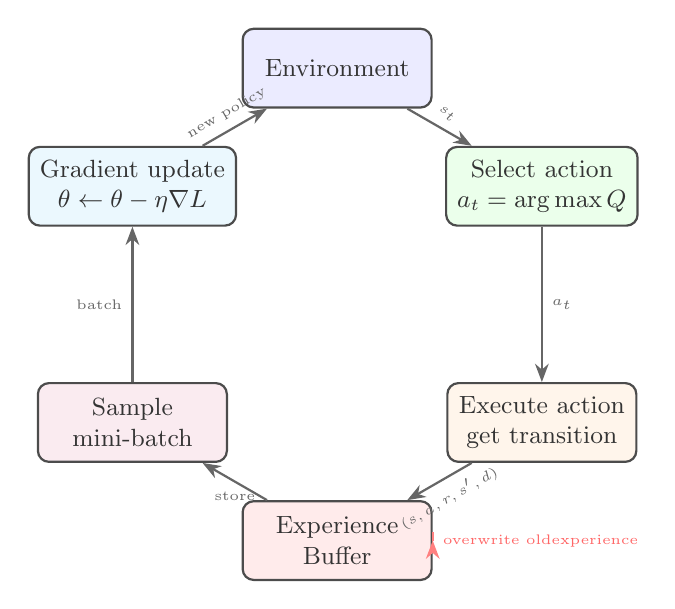
\begin{tikzpicture}[
    node distance=2.2cm,
    box/.style={
        rectangle, rounded corners=4pt,
        draw=black!70, thick,
        fill=white,
        text=black!80,
        font=\small,
        align=center,
        minimum width=2.4cm,
        minimum height=1.0cm,
        inner sep=4pt,
    },
    arrow/.style={
        ->, >=Stealth, thick, black!60,
    },
    label/.style={
        font=\tiny, black!60, midway,
    },
]

% 6 nodes in a hexagon layout
\node[box, fill=blue!8] (env) at (0, 3) {Environment};
\node[box, fill=green!8] (select) at (2.6, 1.5) {Select action\\$a_t = \arg\max Q$};
\node[box, fill=orange!8] (interact) at (2.6, -1.5) {Execute action\\get transition};
\node[box, fill=red!8] (buffer) at (0, -3) {Experience\\Buffer};
\node[box, fill=purple!8] (sample) at (-2.6, -1.5) {Sample\\mini-batch};
\node[box, fill=cyan!8] (update) at (-2.6, 1.5) {Gradient update\\$\theta \leftarrow \theta - \eta \nabla L$};

% Arrows with labels
\draw[arrow] (env) -- (select) node[label, above, sloped] {$s_t$};
\draw[arrow] (select) -- (interact) node[label, right] {$a_t$};
\draw[arrow] (interact) -- (buffer) node[label, below, sloped] {$(s,a,r,s',d)$};
\draw[arrow] (buffer) -- (sample) node[label, below] {store};
\draw[arrow] (sample) -- (update) node[label, left] {batch};
\draw[arrow] (update) -- (env) node[label, above, sloped] {new policy};

% Extra annotation: the "overwrite" dashed loop on buffer
\draw[->, >=Stealth, dashed, red!50, thick]
    (buffer.east) to[out=0, in=-30, looseness=4]
    node[right, font=\tiny, red!60] {overwrite old\\experience}
    (buffer.east);

\end{tikzpicture}
\end{document}
